% !TeX spellcheck = de_CH_frami

\section{Graphen\label{sec:sgwt:graphs}}
\rhead{Graphen}

Unsere Grundlage, auf der wir die SGWT aufbauen wollen, stellen Graphen dar. 
Ein Graph $G$ setzt sich aus Kanten $E$ und Knoten $V$ zusammen.
\begin{equation*}
G = \{V, E\}
\end{equation*}
Eine Kante verbindet dabei jeweils zwei Knoten miteinander.
\begin{equation*}
E = (V_1, V_2)
\end{equation*}

\begin{figure}
    \centering
    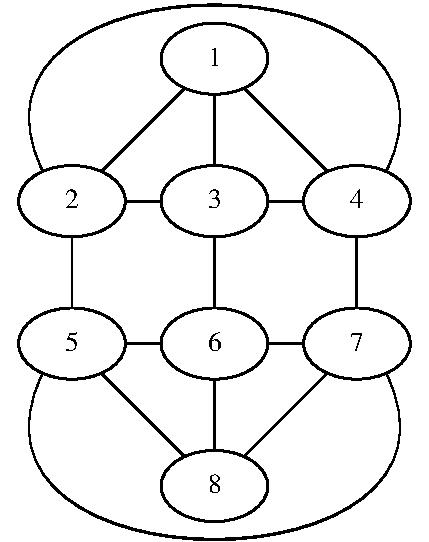
\includegraphics[
        scale=0.7
    ]{papers/sgwt/images/sphere-graph.pdf}
    \caption{Graph Approximation einer Kugel.
    \label{fig:sgwt:sphere:graph}}
\end{figure}

\begin{figure}
    \centering
    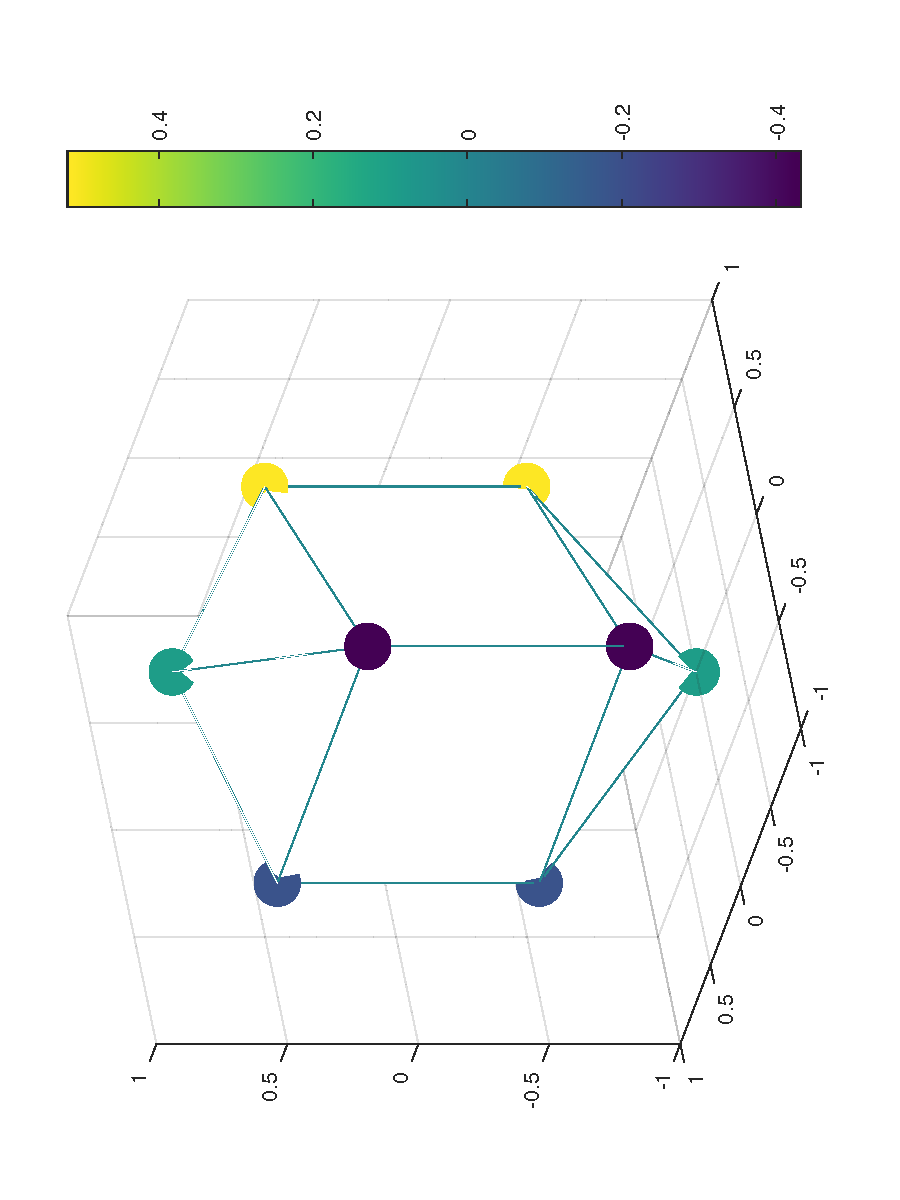
\includegraphics[
        angle=-90,
        origin=c,
        scale=0.7
    ]{papers/sgwt/images/graph-chi-4.pdf}
    \vspace{-80pt}
    \caption{Dreidimensionale Darstellung des Kugelgraphen. Die Funktionswerte 
    werden dabei mit Farben auf den Knoten dargestellt. 
    \label{fig:sgwt:sphere:graph:chi}}
\end{figure}

\begin{figure}
    \centering
    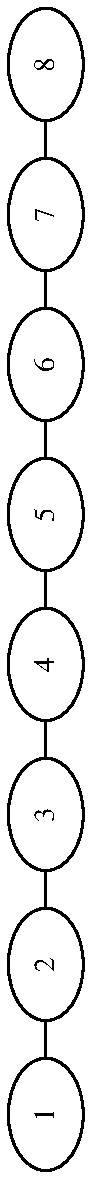
\includegraphics[
        angle=-90,
        origin=c,
        scale=0.7
    ]{papers/sgwt/images/line-graph.pdf}
    \vspace{-200pt}
    \caption{Graph Approximation einer eindimensionalen Funktion. 
    \label{fig:sgwt:line:graph}}
\end{figure}

\begin{figure}
    \centering
    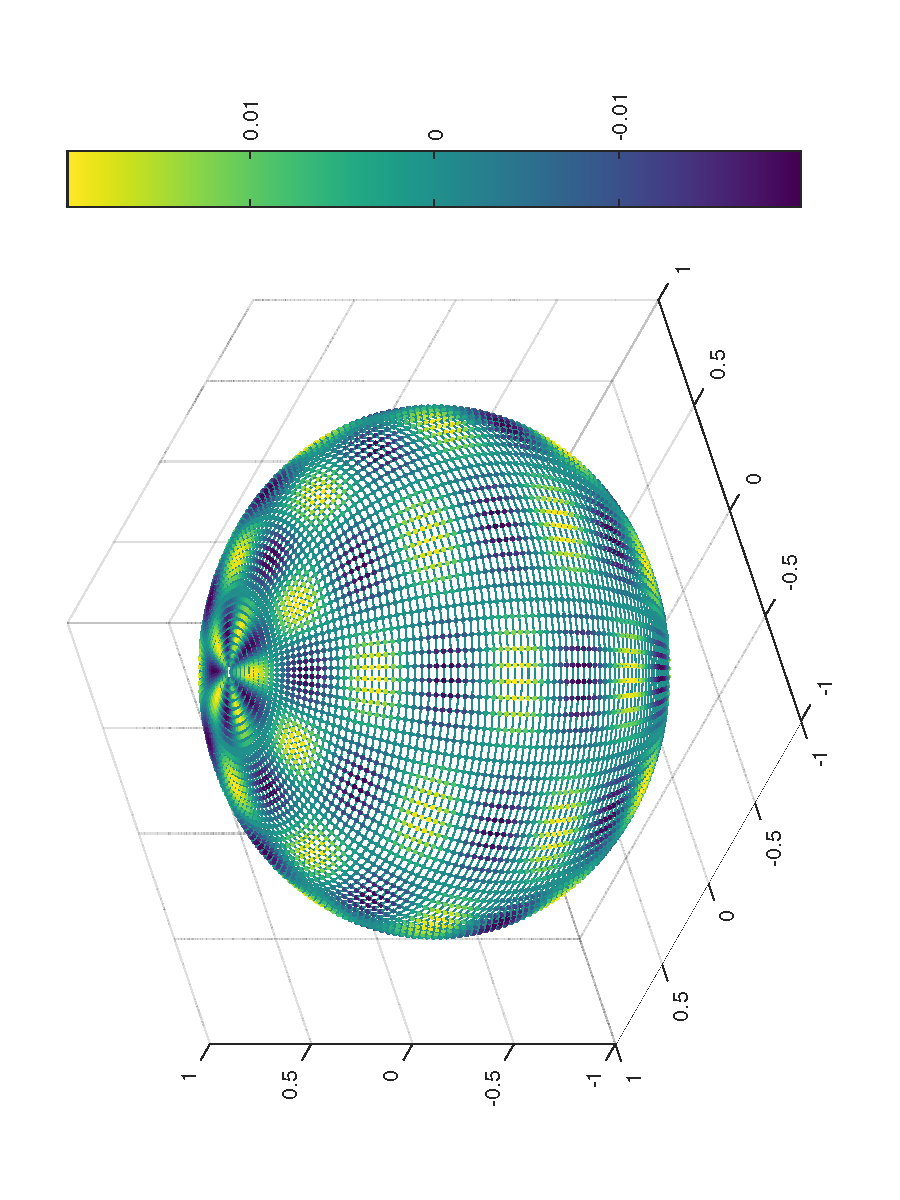
\includegraphics[
        angle=-90,
        origin=c,
        scale=0.7
    ]{papers/sgwt/images/graph-100-100-chi-150.pdf}
    \vspace{-80pt}
    \caption{Kugelgraph mit $l = b = 100$. Darstellung von $\chi_{150}$.
    \label{fig:sgwt:sphere:graph:chi:hh}}
\end{figure}

\begin{figure}
    \centering
    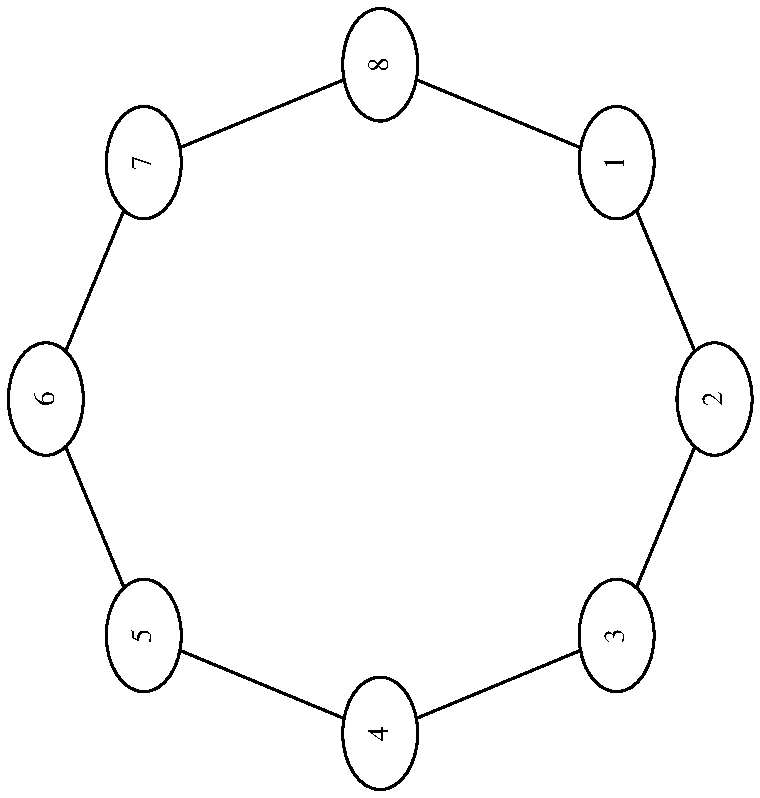
\includegraphics[
        angle=-90,
        origin=c,
        scale=0.7
    ]{papers/sgwt/images/ring-graph.pdf}
    \caption{Graph Approximation einer periodischen eindimensionalen Funktion. 
    \label{fig:sgwt:ring:graph}}
\end{figure}

